\documentclass{rapport}
\usepackage[utf8]{inputenc}
\usepackage{multicol}
\usepackage{pifont} % Pour les symboles appelés par la macro \ding
\usepackage{url} % Comme son nom l'indique, pour les url...

\usetikzlibrary{positioning} % Bibliothèque tikz pour positionner des nœuds relativement à d'autres

\usepackage[colorlinks, citecolor=red!60!green, linkcolor=blue!60!green, urlcolor=magenta]{hyperref} % Pour que les liens soient cliquables. Les options permettent de mettre les liens en couleur.

\usepackage{algorithm}
\usepackage{algo}
\usepackage{colorationSyntaxique}
\usepackage[linguistics]{forest}
\usepackage{tikz}
\usepackage{tabto}
\usepackage[toc,page]{appendix}
\usepackage{geometry}
\setlength{\parindent}{0pt}

\englishTitlePage % Décommenter pour une page de titre en anglais

\pagestyle{fancy}
\renewcommand{\sectionmark}[1]{\markboth{\thesection.\ #1}{}}
\fancyfoot{}

\fancyhead[LE]{\textsl{\leftmark}}
\fancyhead[RE, LO]{\textbf{\thepage}}
\fancyhead[RO]{\textsl{\rightmark}}

\def\Latex{\LaTeX\xspace}
\def\etc{\textit{etc.}}


\title{An AI for Seasons}
\author{Batisse Dylann, Pietrzak Raphaël, Sabatier Juliette, Schmied Margaux}
\supervisor{Pelleau Marie, Renevier Philippe}
\date{Second semester of the year 2021-2022}


\begin{document}

    \maketitle
    
    \clearpage
    \tableofcontents
    
    \newpage
    \begin{abstract}
    The objective of the TER project was to develop different types of AI. We decided to implement AIs based on the Strategy pattern, an adaptive strategy and an AI based on the Monte Carlo algorithm.\\
    We will start with a reminder of the rules and a short description of the version of the Seasons we used. Then we'll describe the implementation of our AIs associated with they performances and the thoughts behind their development.
    \end{abstract}
    
    

\part{Version of Seasons}
    
    Compared to the PD/GL, our version of Seasons isn't much different. 
    We fixed the bugs we may have encountered but we didn't add any card. 

    \paragraph{Goals of the game}
    
        In order to win the game, the players have to gain more prestige points than the others.
        To do that, they have cards, energies, crystals and invocations points at their disposition.
        Each turn of the game, the player can choose a die which can give him a card, energies or other elements. They can use their invocation points, energies and crystals in order to summon cards which can have special effects on the game, or crystallize their energies which gives them crystals that can be converted in prestige points at the end of the turn.

    \section{Progress of the game}
    
        \subsection{Distribution of the cards}
            First of all, for the distribution of the cards at the beginning of the game, a certain amount of cards is given to each player. This amount is the result of the multiplication of the number of years by the number of cards per year given in the game parameters. After that, the players can choose how they want to organize their card for each year.
            Once all of that is done, the processing of the game turns can begin.
        
        \subsection{Description of a turn of the game}
            The first step of a turn is the choice of the dice. The dice are rolled and the players will choose the die they prefer one by one according to the turn order. One die will remain, its use will be described few lines below.
            After every player got their die, they will execute their turn, still following the turn order.
            Once the players all played their respective turn, the cursor on the board indicating the advancement of the game moves forward of a number of steps indicated on the remaining die from the first part of the turn.
            At the end of each turn, the order shifts so the first players becomes the last one, the second player becomes the first one, etc.
        
        \subsection{Description of a turn of a player}
            The turn of a player starts with the player receiving what the die he chose can give him. However, if the player possesses the card "Dice of Malice" on his board, he can decide to re-roll his die before receiving its advantages.
            Then if his die indicates he can draw a card, the player can choose to use a bonus in order to draw a second card and choose which one he prefers between the two.
            
            After that he can choose the actions he will execute during his turn.
            
            \paragraph{Crystallize an energy}
            The player can choose which energy he wants to crystallize if has any in his inventory. This action requires to have a die which gives the right to crystallize, or to have used a bonus with the same effect.
            Depending on the season where is the cursor of the game, each energy return a different number of crystals. For example during the summer a fire energy return 1 crystals but a wind energy return 3 crystals.
            
            \paragraph{Summon a card}
            The player summons a card if he can afford the price. The said price can come in the form of energies or crystals. Finally, the  player will also need to have enough space on his board to summon the card.
            If the card has a direct effect, it is immediately applied. Otherwise the effect will be applied at the right time depending on the effect of the card.
            
            \paragraph{Use a Bonus}
            The player can choose a bonus in a list of available bonuses. The one allowing to draw an additional card is not available as it can only be used in certain conditions.
            Upon choosing the bonus "Crystallize", the player will be granted the right to crystallize at any time in the turn.
            If he chooses the bonus "Gain Invocation Point", he will get one more invocation point.
            If he decides to use the bonus "Change Energy", the player will have to choose an energy from his stock in order to exchange it for another energy he will have chosen.
            
            \paragraph{Activate a card}
            If the player's board contains cards which effect requires to be activated by the player, and if the players can afford to activate at least one of them, he can do so by picking this action.
            
            \paragraph{Do nothing}
            The player ends his turn by doing nothing.
        
        \subsection{End of the game}
            When the cursor reaches the end of the last season of the last year, it's the end of the game. Each player's points will be calculated and the winner(s) will be decided.
            
            First of all, each crystal earned by the player gives him 1 prestige point.
            Then each card on the player's sees its value (indicated on it) being added to the total score of the player. Some cards even have an effect that gives additional prestige points at the end of the game.
            After that for every remaining card in the hand of the player, we remove 5 points of the calculated score.
            And finally if the player used 1 bonus, we remove 5 points, if he used 2 bonuses, 12 points and if he used 3 bonuses, 20 points.
            
            In the end the winner is the player with the most prestige points among the players. It's to have several players with the same amount of crystals, in which case the game ends in a draw between all those players.
        
    \newpage
    \section{Cards}
    The implemented cards are the first thirty cards of the game.
    
    \begin{multicols}{2}
    \begin{itemize}
        \item Amulet Of Air
        \item Amulet Of Fire
        \item Amulet Of Earth
        \item Amulet Of Water
        \item Balance Of Ishtar
        \item Staff of Spring
        \item Temporal Boots
        \item Purse Of Io
        \item Divine Chalice
        \item Syllas The Faithful
        \item Figrim The Avaricious
        \item Naria The Prophetess
        \item Wondrous Chest
        \item Beggar's Hom
        \item Die Of Malice
        \item Kairn The Destroyer
        \item Amsug Longneck
        \item Bespelled Grimoire
        \item Ragfield's Helm
        \item Hand Of Fortune 
        \item Lewis Greyface
        \item Runic Cube Of Eolis
        \item Potion Of Power
        \item Potion Of Dream
        \item Potion Of Knowledge
        \item Potion Of Life
        \item Hourglass Of Time
        \item Scepter Of Greatness
        \item Olaf's Blessed Statue
        \item Yjang's Forgotten Vase
        
    \end{itemize}
    \end{multicols}

\section{Game configuration}

The game can be modified with different parameters described below:

\begin{verbatim}
-MCDepth N        : Depth for Monte Carlo(default: 12)
-MCNbAction N     : Number of action for Monte Carlo (default: 17)
-MCNbBranch N     : Number of branch for Monte Carlo (default: 6)
-logger N         : Game logger (default: 0(false))
-nbCardsPerYear N : Number of cards per year (default: 3)
-nbCaseByYear N   : Number of Case by year (default: 3)
-nbGame N         : Number of games (default: 1000)
-nbPlayer N       : Number of player (default: 2, > 1 and < 5)
-print N          : Print details of games (default: 1(true))
-stats N          : Collect statistics about games (default: 0(false))
-years N          : Number of year per game (default: 3)
\end{verbatim}

    
    
\part{Guarantee AI : Composition of Strategies}

    \section{Description}
    
    For the guaranteed AI we decided to extend what we had already begun to implement during the PD/GL course, which is the Strategy pattern.
    We created different types of strategy for every action (or category), each one being specialized in one type of decision. For each type we can create a player that focuses on one thing. For example crystallizing as much as possible, trying to summon as many cards as possible, or more complex choices like focusing on using combos.
    With that in place, we could create a way to compose a player's strategy, so it could adapt its way of "thinking" depending on the context by switching from a strategy to another.
    The context under which a player must use a strategy or not is defined when we create the player and add the strategy. If the context associated with the strategy is respected, then the said strategy is applied. Else it switches to the next strategy we gave him.
    
    \section{Strategies}
    
    During a game of Seasons, the player has a lot of choices to make and they are very different, he may choose a dice, a card or decide what to do during his turn.
    With that in mind, we decided to implement different types of choice, in order to make good strategies for each type of choice.
    
    
    \subsection{Shape of a strategy}
    
        An abstract strategy contains two fields: a \textbf{nextStrategy} of the same type and a Context \textbf{context}.
        It contains a method \textbf{doChoose}, which is the one that is called in order to use the strategy. It checks if the context is corresponding, and if it does it calls the method \textbf{choose} which actually makes the choice. This method can either return the choice of the player or a \textit{null}.
        If the context does not correspond or if the method \textbf{choose} returns \textit{null}, the method \textbf{doChoose} of \textbf{nextStrategy} is called.
        
        The strategies of a same category extend the corresponding abstract strategy and override the method choose which allows us to define different kinds of choice.
    
    \newpage
    \subsection{Categories of strategy}
    
        \paragraph{ChooseBonus}
        This category contains the strategies defining how a player will decide which bonus to choose from those available.
        
        \paragraph{ChooseCardBetweenMultipleToGet}
        This category contains the strategies defining which card a player will keep when choosing between several different cards. It is used with the bonus allowing to draw two cards, the cards \textit{Divine Chalice} and \textit{Amulet of Fire}.
        
        \paragraph{ChooseCardComeBackInHand}
        This category contains the strategies defining which card to choose from the player's board which is going to come back in his hand. It is used with the effect of the card \textit{Amsug Longneck}.
        
        \paragraph{ChooseCardForInitHand}
        This category of strategies contains every way of choosing how the player wants to organize his cards for the different years at the beginning of the game.
        
        \paragraph{ChooseCardNariaLaProphetesse}
        This category of strategies contains every way of choosing which card to keep and which card to give to the other players when using the card \textit{Naria The Prophetess}.
        
        \paragraph{ChooseCardToDelete}
        This category contains the strategies defining how the player will choose the card to sacrifice when a player uses the card \textit{Syllas The Faithfull}.
        
        \paragraph{ChooseCardToSummon}
        This category contains the strategies defining how a player will choose which card he will summon from his hand.
        
        \paragraph{ChooseCardToSummonForFree}
        This category contains the strategies defining how a player will choose which card he will summon from his hand for free. It is used when the player sacrifices the card \textit{Potion Of Dream}.
        
        \paragraph{ChooseCardToActivate}
        This category contains the strategies defining how a player will choose which card he will activate from his board.
        
        \paragraph{ChoosePlayerEnergyToCopy}
        This category contains the strategies defining how a player will choose another player in order to copy his stock of energies when using the card \textit{Lewis Greyface}. 
        
        \paragraph{ChooseDice}
        This category contains the strategies defining how a player will choose a die between the dice proposed in the game on every turn. 
        
        \paragraph{ChooseEnergyToCrystallize}
        This category contains the strategies defining how a player will choose the energy from his stock he will crystallize.
        
        \paragraph{ChooseEnergyToGet}
        This category contains the strategies defining how a player will choose which energy to get. It is used with the cards \textit{Beggar's Hom}, \textit{Bespelled Grimoire}, \textit{Potion Of Knowledge}, \textit{Hourglass Of Time}, \textit{Yjang's Forgotten Vase}, \textit{Amulet Of Water} and the bonus which allows to exchange an energy for another.
        
        \paragraph{ChooseEnergyToReduce}
        This category contains the strategies defining how a player will choose which energy to remove from the cost of a card, which is the effect of the card \textit{Hand Of Fortune}.
        
        \paragraph{ChooseEnergyToThrow}
        This category contains the strategies defining how a player will choose which energy to throw out of his energy stock. It is used when a player earns an energy but has a full energy stock, with the card \textit{Kairn The Destroyer} when he has to spend an energy, and with the bonus which permits to exchange an energy for another.
        
        \paragraph{ChooseNbDeplacementSeason}
        This category contains the strategies defining how a player will decide where he wants to move when he uses the card \textit{Temporal Boots}. This strategy uses strategy ChooseGoToTheNextSeason, ChooseGoToThePreviousSeason and ChooseStayInTheSeason.
        
        \paragraph{ChooseStayInTheSeason}
        This category contains the strategies defining how a player will decide if he want to stay in the actual season.
        
        \paragraph{ChooseGoToTheNextSeason}
        This category contains the strategies defining how a player will decide if he want to go in the next season.     
        
        \paragraph{ChooseGoToThePreviousSeason}
        This category contains the strategies defining how a player will decide if he want to go in the previous season.  
        
        \paragraph{ChoosePlayerAction}
        This category contains the strategies defining how a player will choose which action he should do during his turn.
        
        \paragraph{ChooseSimilarEnergyToDelete}
        This category contains the strategies defining how a player will choose which type of energy to delete when the player has to delete several energies of a same type. It is used when the player uses the card \textit{Balance Of Ishtar}.
        
        \paragraph{ChooseToKeepDrawnCard}
        This category contains the strategies defining how a player will choose whether he keeps the card he has drawn or not. It is used a the begin of the turn of the player if he has the option to draw a card on his die.
        
        \paragraph{ChooseToUseBonusCard}
        This category contains the strategies defining how a player will decide if he chooses to use the bonus "draw two cards instead of one" when he gets the card from the die at the beginning of his turn. 
        
        \paragraph{ChooseUseDeDeLaMalice}
        This category contains the strategies defining how a player will decide if he uses the card "Die of Malice" when he has it on his board, at the beginning of his turn.
        
    \newpage
    \section{Comparator}
        Most of the time, when we implements strategies we need to compare different objects in order to determine which is the better. So to facilitate this comparison we creates multiples classes implementing Comparator.
        We have multiple type of comparator such as one which compare how much prestige point a card can give, which card is the best given by a list of the best card, etc...
        
        Alongside we also make some classes (singleton) which contains methods to compare more precisely. This classes are mostly used to compare card or energies with predefined list, like a list of energies sort by the most expensive in the actual season.
        
    
    
    \section{Player Factory}
        We created a Factory in order to create different types of AI easily. When we call the method \textbf{getPlayer(playerType, name)} of an object \textit{PlayerFactory}, the method creates a player with a strategy making random choices for each category. Then we enter a switch case which will set some (if not every) strategies to a different one according to the \textit{TypeAIPlayer} given in parameters.
        For example : \textbf{player.setChooseDice(new ChooseDicePrefCristallize())}
    
    
    \section{Context}

        \textit{IContext} is a class which represents an object containing a lambda expression. It contains a function \textbf{isVerified()} which triggers the contained lambda expression.
        Context is a container class, it stores static variables of type \textit{IContext} which contain a lambda expression with a Player as parameter.
        When we call the method \textbf{isVerified()} on a variable contained in the class Context, it gives us the result of the lambda expression.
        It allows us to get information about the game only by using this method.
        
        If we want to know if a player has more than 6 energies, we create the variable \textbf{static IContext moreThan6Energies = (player) -$>$ player.getFacadeIA().getEnergyStock().size() $>$= 6;} and then call \textbf{moreThan6Energies.isVerified()}.
        
        The contexts are used to know details about the advancement of the game and determine if a strategy should be used or not.
            
    \newpage
    \section{Implementation of players not composed}
    
        A player which is not composed always follows the same type of strategy.
        Every strategy implemented in the different categories aim to the same purpose.
        For example \textit{ChooseDicePrefCrystallize} will choose a die which gives the right to crystallize and \textit{ChoosePlayerActionPreCrystallize} will choose the action \textit{Crystallize} if it is available can.
        
            \paragraph{Choose First}
            This player only chooses the first choice from all those available. Mostly used during the development to test some methods.
            
            \paragraph{Random}
            This player makes every choice randomly no matter what.
            
            \paragraph{Pref Crystallize}
            This player chooses whatever can earn him crystals immediately.
            
            \paragraph{Pref Card Point}
            This player will always try to get as many points as possible at the end of the game, mainly by summoning cards with a high prestige point value.
            
            \paragraph{Pref Invocation}
            This player will always try to summon as many cards as possible.
            
            \paragraph{Combos}
            This player will attempt to form combos with his cards and his actions.
            
            \paragraph{Malus}
            This player chooses actions which can handicap other players, for example summon a card which will steal their energy. 
            
            \paragraph{Time Random}
            Time strategy will do everything to play with time, thanks to a die. Its choice between going forward or backward is random.
            
            \paragraph{Time First}
            Time First strategy will always try to stay in the current season.
            
            \paragraph{Time Crystallize}
            Time Crystallize will always try to be in the season in which its energies will be the most valuable.
            
            \paragraph{Time Invocation}
            Time Invocation will try to go forward if its hand is empty and backward otherwise.
            
            \paragraph{Activate}
            This player will try to activate his cards on his board every time he can.
            
            \paragraph{Pref Permanent}
            This player will use cards with a permanent effect as much as possible. A permanent effect can triggered during the whole game (for example each seasons, each end of turn).
        
        \section{Implementation of players composed}
        
        \subsection{Composition on the player factory}
                
            The goal of the composition is to use certain strategies in a certain context, and use some other in a different context, or if the first strategy doesn't give result, use the next one.
            
            In order to do this, when we create a player on the \textit{PlayerFactory} we can set a type of strategy with a composition of different types of strategies.
            A composed strategy look like:

            
            \paragraph{Strategy1()}
                When the strategy is created like this, the player will always use the strategy1.
                If this strategy doesn't return a result, the Random Strategy will be use.
            
            \paragraph{Strategy1( Context1, Strategy2())}
                When the strategy is created like this, the player will check if the context1 is verified, if it's the case the Strategy1 will be used, if not the Strategy2 will be applied.
                If the context1 is verified and the strategy1 doesn't give any result the strategy2 will be used.
            
            \paragraph{Strategy1(Strategy2())}
                Created that way, the player will always try to use the Strategy1. If it doesn't return any result, the Strategy2 will be applied.
            
            \paragraph{How does it work}
            The inheritance of a type of strategy is like this:
            
            \begin{figure}[H]
                \centering
                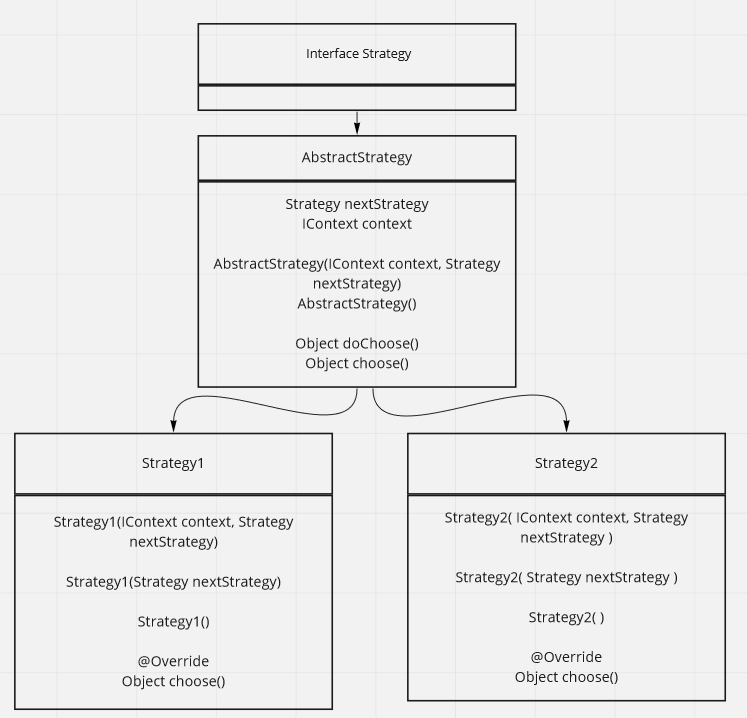
\includegraphics[scale=0.42]{rapport/images/graphics/graph_strategy.png}
                \caption{Schema of the inheritance of a strategy}
            \end{figure}
            
            
            When a choice is required from the player, he will call the method doChoose() in the first strategy in the corresponding composition.\\
            
            \underline{Strategy1()}: \textbf{doChoose()} will call the method \textbf{choose()}, which will return a result to \textbf{doChoose()} which will then return the result to the game. \\
            
            \underline{Strategy1(Strategy2())}: \textbf{doChoose()} of strategy1 will call the method choose() of strategy1.
            If this method return a result, \textbf{doChoose()} of strategy1 will return its result to the game, if not it will call the \textbf{doChoose()} of strategy2 which will then ask a result to the choose() method of strategy2.\\
            
            \underline{Strategy1 (context1, Strategy2())}: \textbf{doChoose()} of strategy1 will verify the context, if is is respected, \textbf{choose()} from strategy1 will be called. Else it will call \textbf{doChoose()} of strategy2.
            
        
            % faire une list ou alors mettre une petit explication sur ce que vous avez voulu faire comment vous avez fait
            \subsection{Compose Raph}
            The initial goal of this AI was to try to create a behavior as close as possible from that of a human. It is using a lot of contexts associated with strategies that would theoretically fit. This AI is detailed in the part \ref{compose_raph_appendix} of the appendix here
            
            
            \subsection{Compose Dyl}
            
            For this composition we try to humanized the AI to make specific choices at certain moment of the game for example we would like to choose a specific dice at the year 1 or 2 or activate the card \textit{Temporal boots} if we are at the last year.  \\
            We tried to adapt the AI behavior against others player but with static choice we could not get the better choice every time because this is a sequence of test that verified the context or not. 
            The AI make choice according to us human, what we would have done if we were playing, we saw by playing ourselves that some moves were better than other. For more details about each strategy and how is it composed see \ref{appendix:compose_dyl_appendix} 
            
            
            
            \subsection{Compose Marg}
            This composition try to reproduce the style of game of Margaux. This player is based on the strategies Pref Card Point and Pref Invocation because they limited the penalty cards at the end of the game. He try to played a little with the time only if he's in the last time to slow down or speed up in function of this hand and he don't crystallized except if is in the last year and last season. We try to arrange strategy to make the best possible player. The players strategies are detailed in the appendix \ref{appendix:compose_marg}.
            
    \newpage
    \section{Performance}
        
        \subsection{How to measure the performances}
            Most of the time when we test our AI we simply run a lot of games with two players and look at the percentage of victory of each player. Sometimes we also look at the number of prestige point gained during a game.
            At first, the games were played against the Random AI, then we eventually used more advanced AI like PrefCardPoint.
            After these tests, we run other games against 3 other AIs to see if the AI is also working and good on a game with 4 players and not only 2.

        \subsection{Not compose AI}
            Our goal with this kind of AI was to make strategies in order to create a great composed AI. We were quite surprised when we saw some of them have a good win rate against the Random AI. For example PrefCardPoint, PrefInvocation and Activate are quite good by themselves as we can see on the figure \ref{fight_images_not_compose_ia}. 
            
            Their efficiency can be explained by the fact that they're using cards more than the other AIs, which results in them having more cards on their boards and less in their hand. In the end they gain more points from their board and lose less from their hand.
            
            We tried different fights between all of our AIs but PrefCardPoint is undoubtedly the best one as shown on the figure \ref{fight_best_img}.

            \begin{figure}[H]
                \centering
                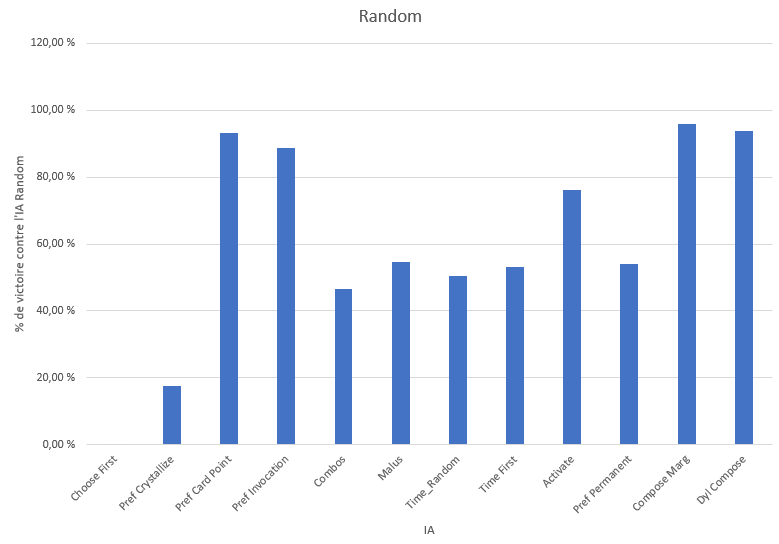
\includegraphics[scale=0.53]{rapport/images/graphics/Guaranteed_IA_against_random.png}
                \caption{Percentage of victory against the Random AI on 10000 games}
                \label{fight_images_not_compose_ia}
            \end{figure}
            
            \begin{figure}[H]
                \centering
                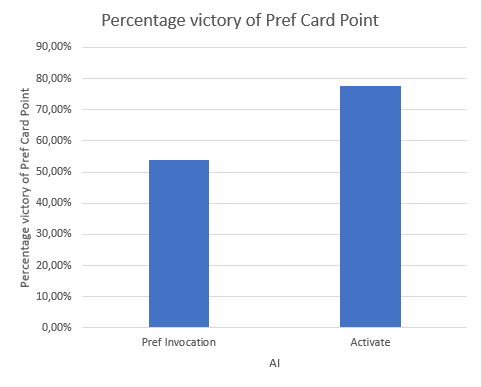
\includegraphics[scale=0.9]{rapport/images/graphics/fight_prefCard_Point.png}
                \caption{Percentage of victory against Pref Card Point}
                \label{fight_best_img}
            \end{figure}
            
        \subsection{AI composed}
            After seeing the performances of the AI which are not composed, it was a bit stressful to make a better AI than PrefCardPoint with a win-rate of 93\% against Random.
            
            
            But with a lot of tests, by composing and modifying each category of strategies, we successfully improved our AI as the figure \ref{fight_against_pref_card_point} highlights, representing the percentage of victory of the composed AI against the AI PrefCardPoint.
            With a win-rate already high for PrefCardPoint the gap is not very big but it is significant enough to see there is an upgrade.
            We tested this strategy against Random, PrefCardPoint and multiple different strategies.
            
            As we can see on the figure \ref{fight_composed_against_other} the composed AI are very efficient, 95\% of victory against random. But also our composed AI are slightly better than the best AI which are not composed, for example ComposeMarg has 57\% of victory against PrefCardPoint. It is not really high but quite good looking at our performance of PrefCardPoints in the figure \ref{fight_images_not_compose_ia}.  
            
            \begin{figure}[H]
                \centering
                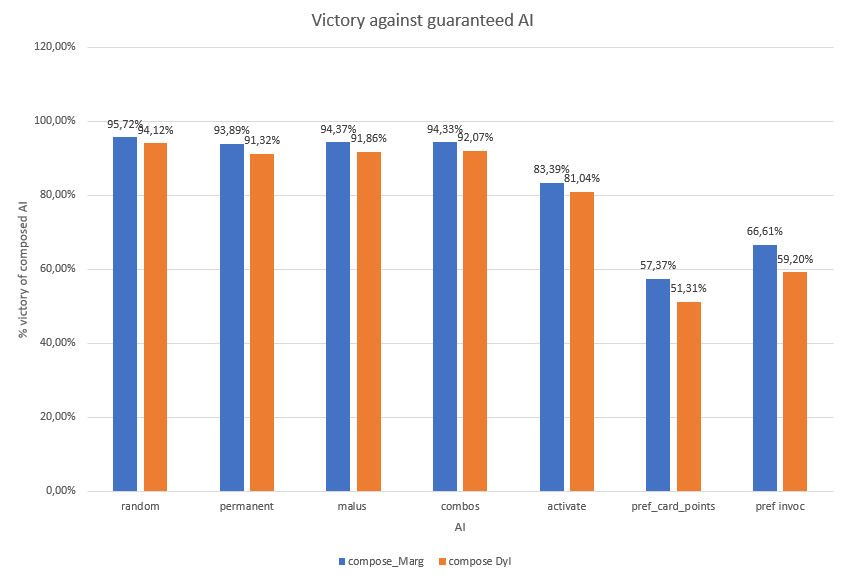
\includegraphics[scale=0.7]{rapport/images/graphics/fight_composed_guaranteed_ai.png}
                \caption{Percentage of victory of Compose Marg and Dyl Compose against other guaranteed AI}
                \label{fight_composed_against_other}
            \end{figure}
            
            \begin{figure}[H]
                \centering
                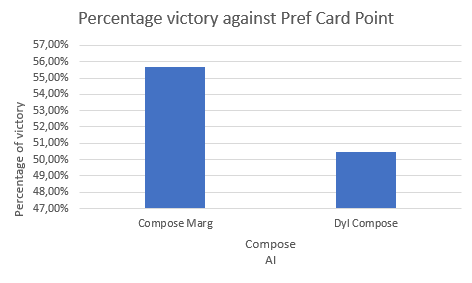
\includegraphics[scale=0.9]{rapport/images/graphics/fight_prefCardPoint_against_composed.png}
                \caption{Percentage of victory against Pref Card Point}
                \label{fight_against_pref_card_point}
            \end{figure}
            
             \begin{figure}[H]
                \centering
                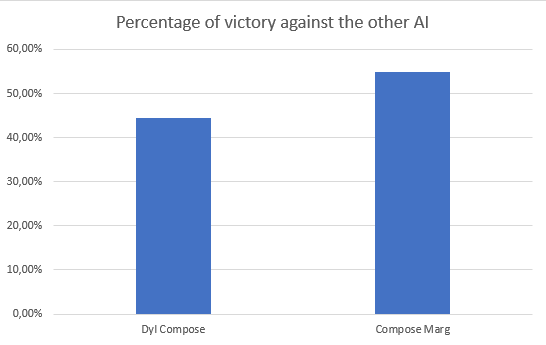
\includegraphics[scale=0.9]{rapport/images/graphics/fight_compose_marg_dyl.png}
                \caption{Percentage of victory against each other}
                \label{fight_compose}
            \end{figure}

    \section{Conclusion of Guarantee AI}
        We took a lot of time developing the guaranteed AI, it wasn't particularly difficult but rather long to implement. We made a lot of different strategies and tried to generalize it as much as we could, which was really time-consuming.
        But at the end the outcome was worth it. We have multiple guaranteed AI which are very good against the random one.
    

    
\part{Ambitious AI Upgraded Guarantee}
        \section{Description}
        Our composition was already very strong and improving it seemed almost like impossible, there were too many specific situations to anticipate not to mention the best behavior would change depending on the AIs we're facing. From these thoughts came the idea of the Adaptive AI, which would decide which way it should behave according to the opponents. The AI would measure each opponent's potential by looking at the cards on their board and the crystals they already own, and pick the one with the highest result. Then it would try to guess the strategy that opponent is using by looking at the type of cards on its board, and finally adapt its own strategy accordingly. The current version of the AI only guesses from the cards on the opponent's board which has a lot of flaws. Once it made its guess, it will copy the strategy it thinks the opponent is using in order to "steal" its choices that would be convenient.
        
        
        \section{Performance}
        The performance are surprisingly low, even though I wasn't expecting big results since it's still in a simple form. It has several flaws, some that can be fixed and some that can't.
        For the latter, it's mainly caused by the way it works: since it tries to guess which strategy an opponent is using, it can't work on composed or Random AI as they constantly use a different one.
        The flaws that can be fixed though, are those such as the poor way it chooses between several possibilities when guessing a type of AI, or the overall way of guessing a strategy which is often wrong. A major one however is that the way the AI works is very limited by itself: since it copies the strategy of the opponent to not leave it room for choices, the opponent automatically does the same, since they're both playing the same way. It can be fixed by changing the strategies the AI uses when focusing on a certain type. That part of the AI is actually its biggest advantage, it can be composed differently depending on the opponents it thinks it's facing.
        
        In short, the AI isn't particularly strong for now but it has a lot of room for improvement, probably more than any AI we currently have. However it can't work against AI that use different strategies in the same game.

\newpage
\part{Ambitious AI Monte Carlo}
        \section{Description}
        In computing, a Monte Carlo algorithm is a randomized algorithm which outputs may be incorrect with a certain probability, generally small. In other words, Monte-Carlo is an algorithm that works on chance, and which computation time is known from the start. However, its outputs may not be the right ones to tackle a problem it's facing, although this is very rare. The advantage of that algorithm is to have low probabilities of failure and to be fast.
        
        \begin{figure}[H]
            \centering
            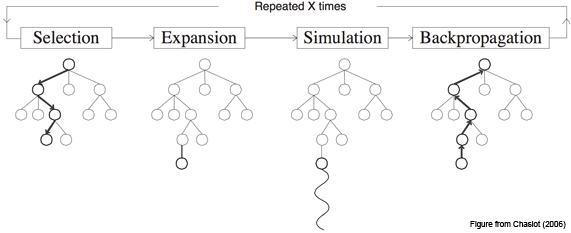
\includegraphics[scale=0.7]{rapport/images/graphics/mcts-algorithm.png}
            \caption{Monte Carlo tree search}
            \label{Monte_carlo_tree_search}
        \end{figure}
        
        
        
        \section{Game cloning}
        Cloning the game is a necessary procedure because when we have to act we have to simulate the game for us and for the other opponents. This operation allows us to keep the state of the game unchanged and pick up where we left off.
        To clone the game we tried to use two methods, one with an external library called \textbf{Gson} and the other one by using the \textbf{Java} built-in interface \textbf{Cloneable}. 
        We have chosen to use the second method because the Gson was not entirely working and the built-in was more advanced.
        
        \subsection{Gson library}
        
        The principle of the \textbf{Gson} library is to make a copy of the whole object even if it's containing other objects. In our case the object that enveloped the whole game is the class GameController and it is the one that we will copy. \\
        How does this method work ? The first thing we need to do is to make a deep copy (copy every nested object) of each object and \textbf{Gson} handles that very easily by transforming an object to JSON format. Once everything is copied we need to load the JSON data to convert them back into real objects with their respective parameters.
        
        \subsection{Built-in Cloneable implementation}
        
        \textbf{Cloneable} is an interface that is used to create an exact copy of an object. Every class used in Monte Carlo algorithm is implementing this interface (Player, Dice, Board, ...). It was necessary to implement the sequence of cloning for example when we clone the DiceSet it also clones each Dice inside. It was an important step because it created infinite loops, we had to be clever to make it work. \textbf{Cloneable} clone well primitives types stored in a class but not others objects so it was necessary to manually add the cloning of these objects.
        
        
        \section{Monte Carlo implementation}
        
        While building our algorithm, we realized that there were many possibilities and that our implementation was creating a stack overflow even though we were trying with few branches and depth. It was necessary to find a solution so we decided to change the type of choice during the simulation. The choices implemented in Monte Carlo of the game are random and do not follow the Monte Carlo algorithm.\\ \\
        As you can see in the figure \ref{Monte_carlo_tree_search}, a traditional algorithm creates a complete tree, but with our changes our algorithm creates a tree that looks like the figure \ref{Monte_carlo_SPBS}. This figure represents the tree behind a choice from our Monte Carlo. The root, representing the function call, will create 5 simulation branches. The first node of each branch is a temporary random choice and its child is a simulation of turns of the game with a depth of 2. In the simulation the die and action are randomly chosen and the other choices are default choices.\\ \\
        Once the algorithm is done with the branch for \textbf{Choice 1}, the choice with the best score is saved, and the branch \textbf{Choice 2} is explored. Upon finishing that branch, the scores of the first choice and of the choice from that branch will be compared, and the best one will be saved. These steps will be repeated until every branch is done.
        \\ \\
        
        
        \begin{figure}[H]
            \centering
            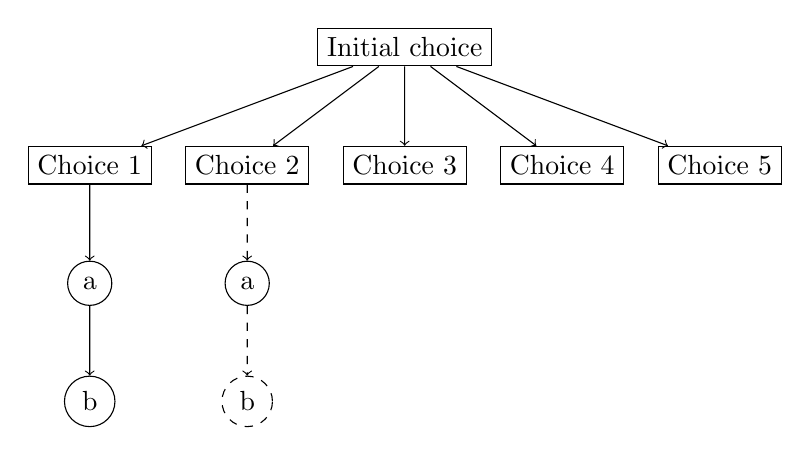
\begin{tikzpicture}[nodes={draw}, ->]
 
            \node{Initial choice}[sibling distance = 2cm]
            child { node {Choice 1} [circle]
                child {node{a}
                    child {node{b}
                        }}}
            child { node {Choice 2} [circle]
                child { node {a} [dashed]
                    child {node {b}}}}
            child { node {Choice 3}}
            child { node {Choice 4}}
            child { node {Choice 5}}
                ;
            \end{tikzpicture}
            \caption{Monte Carlo SPBS}
            \label{Monte_carlo_SPBS}
        \end{figure}


        \subsection{Hand initialization}
        
        During the guaranteed AI part, we saw that the initialization of the player's hand was important for the win-rate. Moreover it is out of any game loop so it seemed easier to start with it.\\
        At the beginning of the game, each player receives 9 cards. When it's an AI Monte Carlo's turn to receive them, we clone the board and the cards. The AI randomly chooses the arrangement of its hand and emulates the choice of the players after it. Then a game is simulated until the end, and this temporary choice with the associated prestige points at the end of the simulated game is saved.\\
        These operations are repeated for the number of connections given in the AI configuration.
        The temporary choice with the best prestige points is selected and returned.
        The real game resumes and the remaining players can initialize their hand.
        
        \subsection{Choosing a dice}
        
        Every time the player wants to choose a dice the algorithm will try several dice and see which one is the best to take at that moment of the game. We chose to make \textbf{Choose Dice} a unique strategy for Monte Carlo because it is a mandatory choice a player will have to make at one point.\\
        When the Monte Carlo player chooses a die the game is cloned and we emulate the random temporary choice of the die. For the players who have to play afterwards we also emulate their choices.The players make their turns and we simulate as many game turns as the depth indicated in the configuration. That is repeated for the number of branches written in the configuration. Then, just like for the initialization, we keep the best temporary choice.
        
        \subsection{Generating the player's actions}
        
        For this part the player's moves for the turn are randomly generated. Basically this method will try multiple moves. For instance we could invoke 3 cards and activate 1 card in the current turn but we will actually try to summon only 1 cards, or none, etc. in a random way. Then we will check which choice was the best to make at the end of the tree search.
        To make this possible we had to create a specific class called MonteCarloTurnLoop which extends PlayerTurnLoop to override how a turn of a Monte Carlo player works and adapt it to our algorithm. In comparison a basic player will make an action until he doesn't want to do anything while Monte Carlo will generate a list of the best actions and then execute it.
        \newpage
        \section{Different versions of Monte Carlo}
        
        \subsection{Random}
        
        This version is a totally randomized algorithm, this means that all the choices the AI will make are randomly tested. For example when the AI wants to crystallize an energy, it will first try to crystallize an earth energy, it can try with fire one, or even with no energy, that choice being random.
        
        \subsection{Heuristic}
        
        After trying a fully random Monte Carlo we decided to add an heuristic to get better results. The heuristic that we used is based on the previous guaranteed AI, with the composed strategies. We still have random choices in this version, particularly in the generation of the moves, the choice of a die and the initialization of the hand like previously stated. For all the other AI choices we used the heuristic from our best guaranteed AI to make it smarter, for example when it comes to summoning a card, we will use the composed strategy.
        
        \section{Performance}
        
        We did some performance testing to see which parameter values are the best for the Monte Carlo Random through our statistics server. For each branch from 1 to 20 and for each depth from 1 to 15 and for each action from 1 to 20, we tested each combination of the parameters on 100 games each time and we took the 3 best win-rates.\\
        On the figures \ref{perf_random} and \ref{perf_monte_carlo_compose}, each point represents an average per observed category. This average is calculated on 100 games with unique parameters.\\
        Both figures are periodic and it can be explained by the rotation of the parameters, when the number of actions is low all curves decrease. With the best parameters, the win rate and the curves for the prestige points and the points of cards are high but the AI does not summon enough cards, so it accumulates too many penalties. We think the problem is that the AI prioritize crystals and leaves energies, and without energies it can't invoke many cards. 
        
        \subsection{Monte Carlo Random}
        
        The figure \ref{perf_random} shows the best results we have for the random Monte Carlo against the random strategy, so the best combination of parameters is 6 branches, depth of 12 and 17 actions.\\
        
        As you can see in the figure \ref{perf_monte_carlo_random_against}, our AI Monte Carlo Random is quite good against not composed AI like Activate, Malus... But although it as 71\% of victory against the random AI, it isn't as good as our composed AI.
        Moreover when we look at the matches between Monte Carlo and the composed AIs, it is obviously not really good with a win-rate below 20\%.
        
        The fact that Monte Carlo is not very good against our best guaranteed AI can be explained by its nature. Monte Carlo is an AI which explores possibilities in the game, but Seasons is a game with a lots of different possibilities and a little choice can change many things. That being said, we decided to keep an AI which take decisions quickly which naturally impacts the research. In order to be faster the AI explores less possibilities and by that fact is less efficient. 
        
        \begin{figure}[H]
            \centering
            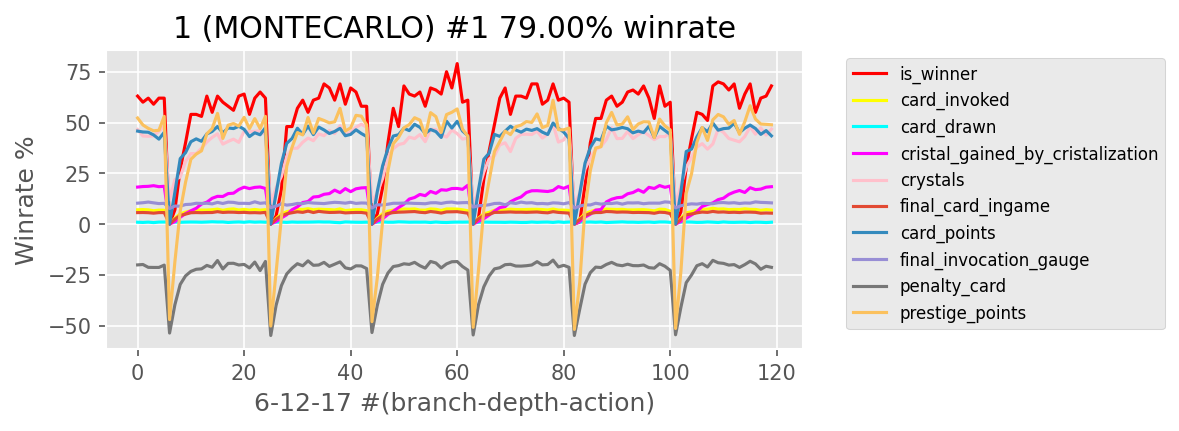
\includegraphics[scale=0.75]{rapport/images/graphics/1 (MONTECARLO)-1555-1.png}

            \caption{Monte Carlo random best parameters \#1}
            \label{perf_random}

        \end{figure}
        
        \begin{figure}[H]
            \centering
            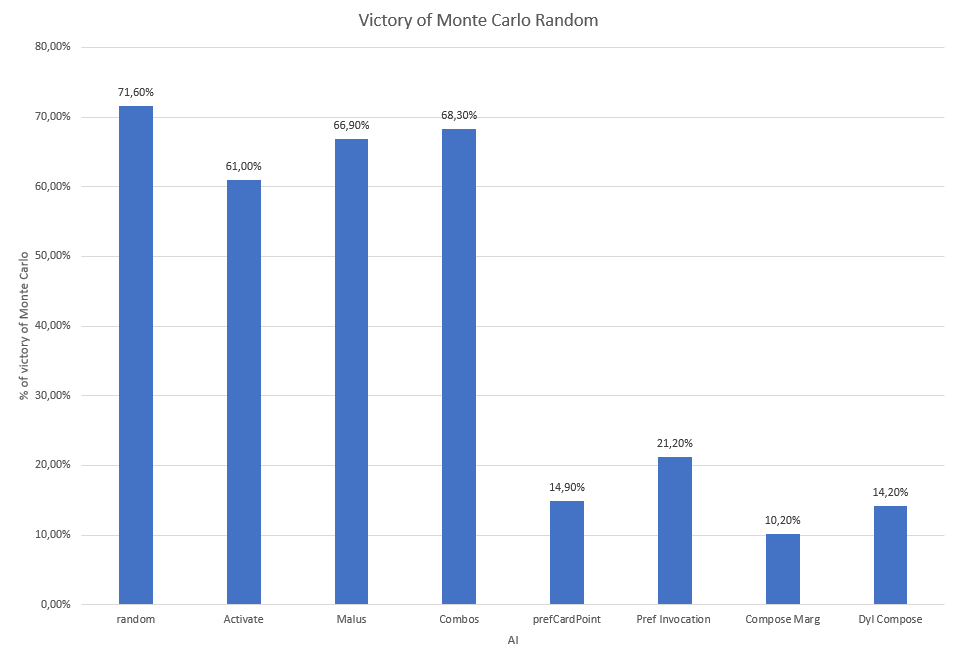
\includegraphics[scale=0.45]{rapport/images/graphics/fight_MT_random.png}
            \caption{Monte Carlo random percentage of victory against other AI}
            \label{perf_monte_carlo_random_against}

        \end{figure}
        
        \subsection{Monte Carlo Heuristic}
        
        As you can see in the figure \ref{perf_monte_carlo_compose} we have a 39\% win-rate against one of the best guaranteed strategies which is \textit{PrefCardPoints}. The best parameters that we found for the heuristic are the following: 5 branches, depth of 4 and 16 actions.\\
        
        The performances of Monte Carlo Compose with these parameters against other strategies are visible in the figure \ref{perf_monte_carlo_compose_against}. The AI wins by a large margin against the strategies Random, Activate, Malus and Combos. We can also see better results than Monte Carlo Random for the strategies Pref Invocation, Pref Card Point, Compose Marg and Compose Dyl. As this AI is based on Compose Marg, we could hope to win at least against Pref Invocation and Pref Card Point. We think the poor performances are caused by the initialization of the hand, since choices are random and during the simulation the choices of the other players are randomly emulated.
        
        
        
        \begin{figure}[H]
            \centering
            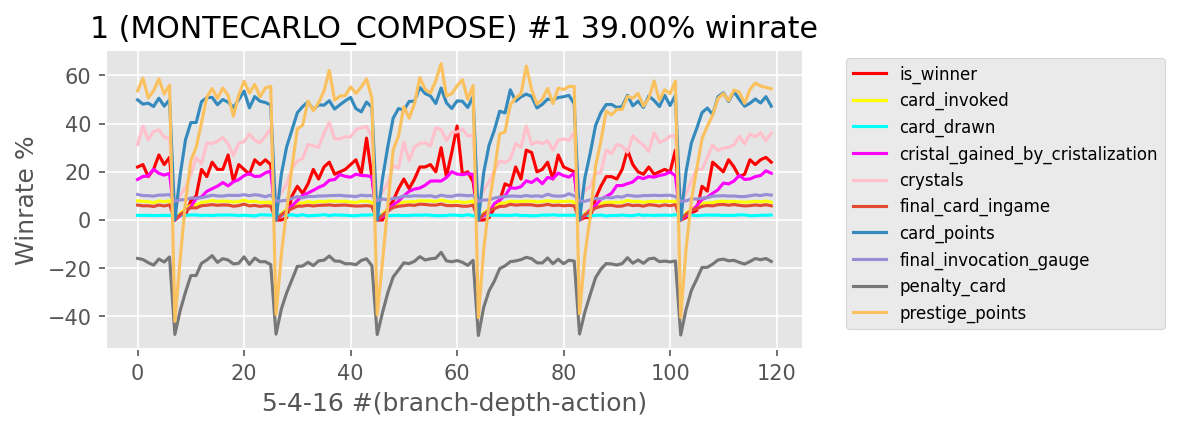
\includegraphics[scale=0.75]{rapport/images/graphics/1_MONTECARLO_COMPOSE-1136-1.png}
            \caption{Monte Carlo heuristic best parameters \#1}
            \label{perf_monte_carlo_compose}

        \end{figure}
        
        \begin{figure}[H]
            \centering
            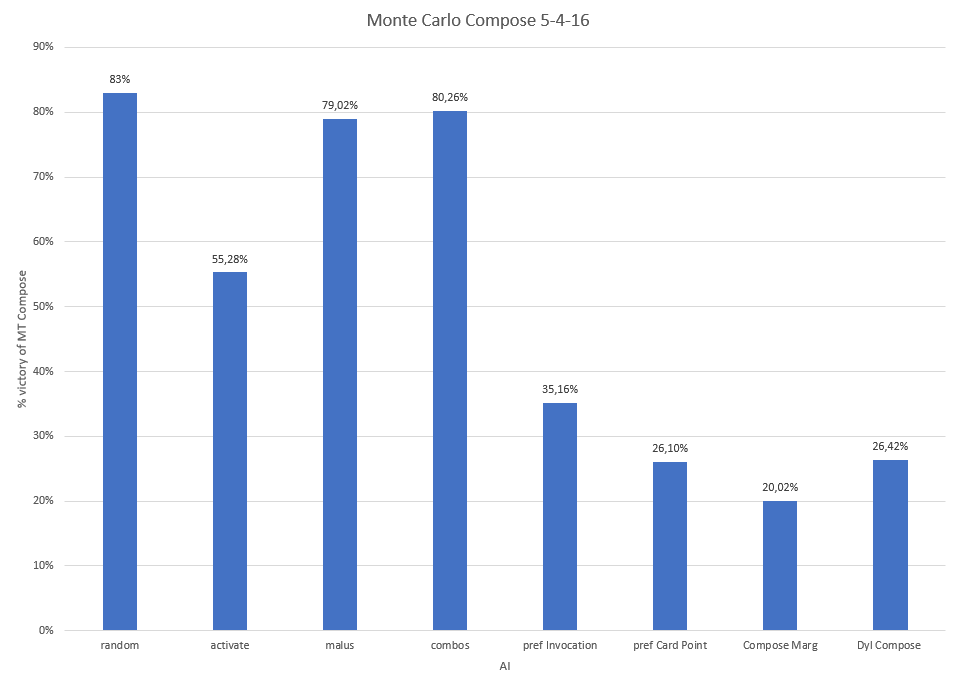
\includegraphics[scale=0.45]{rapport/images/graphics/fight_MT_COMP_5_4_16.png}
            \caption{Monte Carlo heuristic percentage of victory against other AI}
            \label{perf_monte_carlo_compose_against}

        \end{figure}
        
   
        
        


        
    

    \part{Issues Encountered}
    \section{Guaranteed AI}
        For this AI, at the beginning we only made a few strategies, and after a while we had a lot of ideas and we wanted to make a lot of strategies. 
        Of course making many strategies took a long time, particularly in November.
        Also the more strategies appeared the more difficult it began to abstract them.
        
        After making a good amount of different strategies to fulfill our goal which was to compose with multiple strategies, it appeared that some of them were already really efficient against the Random AI. The difficulty that occurred when we began to compose our own AI was to make a better AI than our classic AI which used only one type of strategy. Making a lot of strategies was really long and for this stage we didn't have much time, but in the end we succeeded at making a better AI.
    
    \section{Ambitious AI}
        \subsection{Another type of Monte Carlo}
            When we were thinking about which kind of ambitious AI we wanted to implement, we had two different ideas of how to implement Monte Carlo.
            But after some time of reflection we decided that it was repetitive and not useful. It was more interesting to choose one, and look for something else.

        \subsection{Reinforcement Learning}
            Reinforcement learning is a type of AI which makes us dream and looks really interesting.
            When we started doing some researches about machine learning, we thought it would be perfect for Seasons. Classic machine learning would have required a huge amount of data which we couldn't have, thus making reinforcement learning a good alternative as it would learn on its own with each game.
            But when we actually tried to implement it, we quickly realized the game was not adapted for it, and we would have had to spent too much time trying to make it work.
            
            So as we were getting short on time, we decided to simply improve already existing strategies until we'd find something good.
        
            
            
    
    

    \part{Summary} 

In the end, this project was one of the most difficult we've ever had. Not because it was particularly difficult but because of how time-consuming and dense it was. The game contains an enormous amount of elements, each one having its own particularity and therefore its load of issues. Putting them all together correctly was already a challenge, and we had to add the Strategy pattern which required a lot of tedious coding.\\

On top of all this, the TER project required a lot of time and reflection because of all the possibilities we had to take in count when creating an AI. While we had first planned to simply implement a Monte-Carlo AI, we hadn't anticipated that being four for that work would've been too much, so we had to improvise another type of AI. In the meantime, the other projects prevented us from focusing on the project as much as we would have wanted to.\\

Despite all those obstacles, we still managed to implement an efficient Monte-Carlo algorithm which wins against most of the basic AIs, and we came up with a simpler AI that has a great potential. However, in spite of our efforts to create an ambitious AI as powerful as possible, the best ones remain the composed AI "Compose Dyl" and "Compose Marg". All these different types of player are working together on the game we created in the previous part of the project.

In fine, this project taught us how complicated it can be to add a sophisticated AI on a game without anticipating it during the development of the said game. Still, we learnt to use new patterns we had never encountered before, and we discovered the Monte-Carlo algorithm which we were quite curious about for a while.
    

    

\appendix

\begin{appendices}
\addtocontents{toc}{\protect\setcounter{tocdepth}{0}}

\section{Compose Raph appendix}\label{compose_raph_appendix}

\paragraph{ChooseCardForInitHand}
First things first, the way it chooses the cards to initialize its hand is the one used by our AI that tries to summon as many cards as possible, because chooses the cards that are easier to summon for the beginning of the game, thus guaranteeing a better start.

\paragraph{ChooseBonus}
When it's time to choose a bonus, it checks if it needs more invocation points, in which case it try to use the bonus to get more. If it needs more or different energies, it will try to pick the bonus to exchange an energy, and if it has less crystals than anyone, it will try to pick the bonus that allows him to crystallize. Else, it won't pick any.

\paragraph{ChooseCardComeBackInHand}
If it has to take a card back into its hand, the AI will check if it has a lot of resources or if it's behind the others score-wise, and if so it will take back the card that would've given less points. However if it doesn't have many resources or if the game is near its end, it will choose a card that is easy to summon back.

\paragraph{ChooseCardNariaLaProphetesse}
When using "Naria the Prophetess", it will always try to pick the card that would give it more points at the end.

\paragraph{ChooseCardToDelete}
If an opponent uses "Syllas the Faithful", the AI will first choose to sacrifice cards that would inflict a penalty to the opponents. If it doesn't have any, it will try to delete a card that doesn't give much points, and finally it will try to remove a card that isn't part of a combo. Now that I think about it, it would've made more sense to make it work the other way around.

\paragraph{ChooseCardToSummon}
When summoning a card, it will try to summon cards that can give a lot of points if it's behind the other players and if the game is about to end. However, if the game's just begun, it will attempt to summon cards applying penalties to the other players, as these cards often work on the long run, it would be the best way to exploit them. These cards would also be summoned if the AI sees it has less crystals than the others, to steal some. If the game isn't at any particular point it will try to use cards with permanent effects, then cards that can be activated and then cards that would let him summon even more cards.

\paragraph{ChooseCardToSummonForFree}
It follows the same logic when summoning a card for free.

\paragraph{ChooseCardsToActivate}
When activating a card, it will try to activate cards that would help it summon more cards if it has too many in its hand, If it notices it has less crystals than the others, it will try to activate "Kairn The Destroyer" in order to steal crystals. If it realizes it has too many energies, not enough crystals and little time before the game ends, it will try to activate cards that would help him crystallizing energies. In other cases it will simply try to activate combos of cards.

\paragraph{ChoosePlayerAction}
One of the most important choice an AI has to make is the set of actions it will perform during its turn. The first thing it will check is if it has one or more cards with a high value in its hand, and it will pick the action to summon if so. It will do the same if it decides it has too many cards in its hand and if it has enough resources to potentially summon something. If it needs crystals and it has a lot of energies, it will try to crystallize if it can.
\\\\
Thinking about all the possible situations takes some time and this AI couldn't be totally completed, some types of strategy are missing and some aren't as good as they should be, as it can happen that a context is verified although it would have been wiser to check another one first.


\section{Compose Dyl appendix}\label{appendix:compose_dyl_appendix}

\paragraph{ChooseBonus}
For this strategy we first try to use a bonus if we need to invoke a card, then we check if we need energies to activate a card.

\paragraph{ChooseCardBetweenMultipleToGet}
When we need to choose a card, we check if the card can create some combos with our hand. If no combo have been found, we choose the card that has the most prestige points. If we can't find any interesting card, we move on to get a card that can helps us getting more cards and finally a card that can be activated.

\paragraph{ChooseCardComeBackInHand}
The player will first try to take a card which would takes him back in time like the \textit{Temporal Boots} if it's the last year of the game. Else he'll take a card that inflicts a penalty on the other players or a card which gives the smallest amount prestige points.

\paragraph{ChooseCardForInitHand}
The player tries to create the best combo, but if he can't, he'll take the cards that cost the least

\paragraph{ChooseCardNariaLaProphetesse}
The player will choose the card that has the smallest cost for himself if the context last year is verified. If not, he'll choose the best combos according to our hand, a permanent card if no combo could be found and in first year context, a card that can be activated if it's the middle of the game and then he'll take the \textit{Temporal Boots} if there is one available.

\paragraph{ChooseCardToDelete}
The player will first look for a card with a permanent effect on the board, if none is found then he'll look for a card that could be activated, then the card that would give the least prestige points, or \textit{Temporal Boots} if there is one and finally we delete a penalty card.

\paragraph{ChooseCardToSummon}
\label{card_to_summon}The player will try to summon the card that would earn him the most prestige points. If a minimal amount of prestige point is not respected, he'll try to invoke the card that costs the least. Then a permanent card if context middle game is verified, a card that can be activated, then a penalty card against the other players, a card with combos if no penalty card is found and finally \textit{Temporal Boots} if we have it.

\paragraph{ChooseCardToSummonForFree}
This strategy is the same as the basic one \ref{card_to_summon}.

\paragraph{ChooseCardToActivate}
The player will try to activate \textit{Temporal Boots} if the game is in its last year, if none is found he'll try to activate the card that would help him get more cards and then activate a card with good combos with what he has in his hand.

\paragraph{ChoosePlayerEnergyToCopy}
We try to copy energy from the player that match the best energies for a permanent card in our hand if we are in the first year, if not we copy the energies that match the best energies for a card that cost the least. Finally if none of these are respected we try to copy the energies from a player that match an activable card in our hand.

\paragraph{ChooseDice}
The player will choose a die to invoke more card if the game is either in year 1 or year 2, if we are in the last year he'll choose one to crystallize and then take a die which would allow him to invoke the card that would give him the most prestige points.

\paragraph{ChooseEnergyToCrystallize}
The player will choose to crystallize an energy if we are in the last year and his hand is empty.

\paragraph{ChooseEnergyToReduce}
The player will choose an energy such that he could invoke more cards.

\paragraph{ChooseEnergyToThrow}
The player will remove the energies that do not match the energies needed for the cards in his hand. If none is found he'll throw the energies required for the card that costs the least, then the energies for the card that has the least combo and finally the energy that would be worth less if he'd want to crystallize it.

\paragraph{ChooseNbDeplacementSeason}
The player will make a decision according to ChooseGoToTheNextSeason, ChooseGoToThePreviousSeason and ChooseStayInTheSeason.

\paragraph{ChooseStayInTheSeason}
The player will choose to stay in the season if his hand is not empty.

\paragraph{ChooseGoToTheNextSeason}
The player will choose to go in the next season if his hand is empty.

\paragraph{ChooseGoToThePreviousSeason}
The player will choose to stay in the season if his hand is not empty.

\paragraph{ChoosePlayerAction}
Player will try to choose the action to invoke more card, otherwise it will take the activable cards.

\paragraph{ChooseSimilarEnergyToDelete}
The player will choose an energy that is not required to summon the card that costs the least, or a card to summon even more cards. If no energy is deleted after with that condition, he'll choose the energy that aren't needed for the cards that can be activated and finally for \textit{Temporal boots}.

\paragraph{ChooseToKeepDrawnCard}
The player will prioritize the permanent cards, the cards that can be activated, the penalty cards, the cards that can create a combo and \textit{Temporal boots}, in that order from the highest priority to the lowest.

\paragraph{ChooseUseDeDeLaMalice}
If the die is not satisfying, in other words if the player had to choose his die by default, he'll use Die of Malice.

\section{Compose Marg appendix}\label{appendix:compose_marg}

    \paragraph{ChooseBonus}
    If the player needs invocation points, he'll take the invocation bonus. He'll pick the crystallization bonus if his energy stock is full, and in other cases, he won't pick any bonus.
    
    \paragraph{ChooseCardBetweenMultipleToGet}
    If the choice is made during the first year, the player will take the card with the highest value. If it's during the second year, he'll take the best one to create a combo, and else he'll take the easiest card to summon.
    
    \paragraph{ChooseCardComeBackInHand}
    The player will look for cards that have an effect upon invocation. If he can't find any, he'll pick the easiest card to summon.

    \paragraph{ChooseCardForInitHand}
    The player organizes his hand in order to create the best combos.
    
    \paragraph{ChooseCardNariaLaProphetesse}
    The player will distribute the cards such that the players with more cards will receive the toughest cards to summon. The players with less cards will receive cards that are easier to summon.
    
    \paragraph{ChooseCardToDelete}
    The player will first try to delete cards with a permanent effect. If he can't find any and if there's a card with a value over 10, he'll try to delete the card with the lowest value. Else he'll choose a card that can be activated.
    
    \paragraph{ChooseCardToSummon}
    During the first year, the player will try to summon cards with permanent effects. Then he'll try to summon \textit{Temporal Boots}, penalty cards or cards with the highest value, in order of priority.
    
    \paragraph{ChooseCardToSummonForFree}
    The player follows the same logic than for ChooseCardToSummon.

    \paragraph{ChooseCardToActivate}
    If he can, the player will activate cards that would help him summon more cards. Otherwise, if it's the middle of the game, he'll try to activate a card that applies a penalty to an opponent, else he'll try to activate a card with a good combo available.
    
    \paragraph{ChoosePlayerEnergyToCopy}
    The player will look for the player with the energy stock that would fit the most to summon valuable cards, or to summon cards that would create a great combo.

    
    \paragraph{ChooseDice}
    If it is the first or second year, and if the player needs invocation points, he'll choose a die that gives invocation point. If it's the last year, he'll take the die which allows him to crystallize. If none of the previous context is verified, he'll take the die with the best energies in order to summon the most valuable card.
    
    \paragraph{ChooseEnergyToCrystallize}
    The player crystallizes the most expensive energy.
    
    \paragraph{ChooseEnergyToGet}
    The player chooses the best energy to summon his most valuable card.

    \paragraph{ChooseEnergyToReduce}
    The player chooses an energy he needs but doesn't possess, or just a random energy.
    
    \paragraph{ChooseEnergyToThrow}
    The player chooses an energy that isn't required to summon a valuable card.

    \paragraph{ChooseNbDeplacementSeason}
    The player will make a decision according to ChooseGoToTheNextSeason, ChooseGoToThePreviousSeason and ChooseStayInTheSeason.
    
    \paragraph{ChooseStayInTheSeason}
    The player will choose to stay in the season if his hand is not empty.
    
    \paragraph{ChooseGoToTheNextSeason}
    The player will choose to go in the next season if his hand is empty.
    
    \paragraph{ChooseGoToThePreviousSeason}
    The player will choose to stay in the season if his hand is not empty.

    \paragraph{ChoosePlayerAction}
    If we're in the last season of the last year he'll try to crystallize his energies, else he'll choose to summon, use a bonus or activate a card, in this order of priority.
    
    \paragraph{ChooseSimilarEnergyToDelete}
    The player deletes the most useless energy to summon a card.
    
    \paragraph{ChooseToKeepDrawnCard}
    If the card is useful to summon more cards, or if it's not the last year and his hand is empty he'll keep the card no matter what.
    
    \paragraph{ChooseToUseBonusCard}
    The player doesn't use his bonuses.
    
    \paragraph{ChooseUseDeDeLaMalice}
    If the die is not satisfying, in other words if the player had to choose his die by default, he'll use Die of Malice.

\end{appendices}

 
\end{document}
